\section{Homophily: \emph{"Birds of a feather flock together"}}
\label{sec:homophily}
%\vspace{-0.2cm}
%\begin{center} \emph{Birds of a feather flock together} \end{center}
%\vspace{0.1cm}

Homophily refers to the tendency of individuals to connect to similar others: two individuals (and thus their corresponding nodes in a social network) are more likely to be connected if they share common characteristics~\cite{mcpherson2001birds,lazarsfeld1954friendship}. The characteristics often considered are inherent to the individuals: they may represent their social status, their preferences, their interest, ... A related notion is the one of {\it assortativity}, which is slightly more general as it applies to any network, and not just social networks, and refers to the tendency of nodes in networks to be connected to others that are similar in some way.

A definition of homophily has been proposed in~\cite{la2010randomization}. However, this definition, which relies on a single characteristic (as age or gender), does not allow one to assess whether latent models for link prediction capture the homophily effect or not. We thus introduce a new definition of homophily below, which directly aims at this:
%
\begin{definition}[Homophily]
	Let $\mathcal{M}$ be a link prediction model as defined above and $s$ a similarity measure between nodes. We say that \emph{$\mathcal{M}$ captures the homophily effect} iff, $\forall (i,j,i',j') \in V^4$:
%
\begin{equation}
s(i,j) > s(i',j')  \implies \pr(y_{ij}=1 \mid \mathcal{M}) > \pr(y_{i'j'}=1  \mid \mathcal{M}) \nonumber
\end{equation}
%
A model which verifies this condition is said to be \emph{homophilic} under the simylarity $s$.
\end{definition}
%
As one can note, this definition directly captures the effect "if two nodes are more similar, then they are more likely to be connected The model $\mathcal{M}$ considered can either be regarded in a purely generative setting, or be learned from the data. The above definition encompasses both cases, the parameters $\mat{F}$ and $\mat{\Phi}$ being either generated or learned. Furthermore, in some cases, for example when one has access to users' interest or social information, one may use \textit{a priori} representations of nodes as well as given weight matrix between them. This situation corresponds to the case where the matrices $\mat{F}$ and $\mat{\Phi}$ are given, the variables $y_{ij}$ still being generated according to Eqs.~\ref{eq:link-ilfm} and \ref{eq:link-immsb}. The definition of homophily given above is still applicable in this setting.

The similarity function assesses to which extent two nodes share the same characteristics. The parameter $\mat{F}$ captures some latent characteristics of the nodes, whereas the parameter $\mat{\Phi}$ captures the correlations between these latent characteristics. In a first approach, one can define for $\M_e$ and $\M_g$, on their basis, a "\emph{natural}" similarity between nodes as follows:
%
\begin{align}
&s_n^{\M_e}(i,j) = \mat{\hat{f}}_{i} \mat{\hat{\Phi}} \mat{\hat{f}}_j^\top \nonumber \\
&s_n^{\M_g}(i,j) = \int_{f_i, f_j,\Phi} \mat{f}_i\mat{\Phi} \mat{f}_j^T \p(f_i, f_j) \p(\Phi) df_{i,j}d\Phi
%\label{eq:natural-sim}
\end{align}
%
It is straightforward that $\mathcal{M}_e$ and $\M_g$ is homophilic wrt to $s$, as $s(i,j)$ corresponds to the probability of generating a link between nodes $i$ and $j$ (Eq.   ~\ref{eq:link-me}). We thus have the following property:
%
\begin{proposition}[] $\M_e$ and $\M_g$ are homophilic wrt the natural similarities respectively  $s_n^{\M_e}$ and $s_n^{\M_g}$.
\end{proposition}

The homophyly define by $s_n$ is trivial because there is a direct mapping between the node similarity and the links likelihood. Though, this proposition carry the idea that we can always choose a node similarity that would conserve the homophily effect but with a loss of interpretability of the similarity metric. An exemple of such conservation is any homothetic transformation of the natural similarity.

Therefore, A more interesting question would be to inspect the homophilic effect with a similarity that only depend os the latent features, that is nearest of the classical notion of homphily in networks. We define a latent similarity between nodes which is decorrelated of $\Phi$, which is associated to the topology of the random graph:

\begin{align}
&s_l^{\M_e}(i,j) = \mat{f}_{i} \mat{f}_j^\top \nonumber \\
&s_l^{\M_g}(i,j) = \int_{f_i, f_j} \mat{f}_i\mat{f}_j \p(f_i, f_j)  df_{i,j}
\label{eq:latent-sim}
\end{align}


\begin{proposition}[]
	ILFM is and IMMSB does not satisfy the latent homophily under the latent similarities respectively $s_l^{\M_e}$ and $s_l^{\M_g}$.
\end{proposition}

\noindent \textbf{Proof} We start in the $\M_g$ setting.
\begin{align*}
&\p(y_{ij}|\M_g) = \int_{f_i, f_j,\Phi} \mat{f}_i\mat{\Phi} \mat{f}_j^T \p(f_i, f_j) \p(\Phi) df_{i,j}d\Phi \\
& = \int_{f_i, f_j,\Phi} (\sum_{kk'}f_{ik}f_{jk'}\phi_{kk'}) \prod_{kk'}p(\phi_{kk'}) \p(f_i, f_j)  df_{i,j}d\Phi
\end{align*}
We have that $\Phi$ are i.i.d either from beta or normal distribution. Thus we have that $\E[\Phi] = \mu \unit$, where $\unit$ is matrix with one everywhere and $\mu$ a constant corresponding to the mean of the prior over weight. Then we have:
\begin{align*}
&\p(y_{ij}|\M_g) =  \mu \int_{f_i, f_j} (\sum_{kk'}f_{ik}f_{jk'})  \p(f_i, f_j)  df_{i,j} \\
&= \mu \int_{f_i, f_j} (\sum_kf_{ik}f_{jk} +  \sum_{k \neq k'}f_{ik}f_{jk'})  \p(f_i, f_j)  df_{i,j}
\end{align*}

We will first treat the case of IMMSB. From the models, and HDP priors we have the following properties:
\begin{align*}
\p(f_i,f_j|\alpha_0, \pi) &= \p(f_i|\alpha_0,\pi)\p(f_j|\alpha_0,\pi) \\
\int_{f_i} f_{ik} p(f_i)df_i &= \alpha_0 \pi_k \qquad \text{avec} \quad \mat{\pi} \sim GEM(\gamma)
\end{align*}
Thus we can rewrite $p(y_{ij}|\M_g)$ such that:
\begin{align*}
p(y_{ij}|\M_g) \propto  \sum_k \pi_k^2 + \sum_{k\neq k'} \pi_k \pi_{k'}
\end{align*}

We see that the definitions is misspecified, because, in mean there is no variation in neither the similarity, or the link probability (as show in the sparstiy section). That why, a similarity based on either the fixed feature makes more sens 

Suppose now, we have $(i,j,i',j') \in E$ such that $s_l^{\M_g}(i,j) > s_l^{\M_g}(i',j')$. We follows that:

We then redefine the homophily that marginalize over weight, (previous definition !), to keep some variability in the homophiy definition.

~\\
(....copy paste..old definition...!?)
~\\

A counter example is as follow, chose $f_i=f_j=(0,1,0)$ and $f_{i'}=(1,0,1)$ and $f_{j'}=(0,1,0)$.Thus we have $s(i,j)=2$ and $s(i',j')=0$, and $p(i,j) \propto 2$ but $p(i',j') \propto 4$. Thus homophily is not satisfied. 








 
%
\begin{align}
&\mathbb{E}_{\Phi}[\pr(y_{ij}=1 \mid \mathcal{M})] \nonumber \\
&= f_i \E[\Phi]f_j = \mu f_i \otimes f_j  \nonumber \\
&= \mu (\sum_k f_{ik}f_{jk} + \sum_{k\neq k'} f_{ik}f_{jk'} ) \nonumber
\end{align}
%
Where $\otimes$ is the outer product. Whitin the last equation, it is easy to find a counter example where the similarity order is lost by the outer product. Example fall in the stochastic block model case (which is a special case of both model), A counter example is as follow, chose $f_i=f_j=(0,1,0)$ and $f_{i'}=(1,0,1)$ and $f_{j'}=(0,1,0)$.Thus we have $s(i,j)=2$ and $s(i',j')=0$, and $p(i,j) \propto 2$ but $p(i',j') \propto 4$. Thus homophily is not satisfied. Finally, note that because the property is false in the global case, it is straightforward to show that the property is also false in the local case   \hfill $\Box$ \\







This proposition means that the latent features generated or learn for both model will not encode the classical vision of homophily, which says that if two individuals have similar feature, they will be likely to connect. This proposition also hilghight the fact the latent feature of iMMSB and ILFM can't be interpreted out of the box as communities where links occur more likely when two individuals has identical membership.

In the contrary, one can imagine that if $\Phi$ is constrained such that latent homophily is true, one can directly interpret the latent features as communities indicator. This is basically what is done is this paper \cite{AMMSB} to find overlapping communities within the MMSB models. The authors renamed the constraint MMSB to a-MMSB, standing for assortative MMSB. \textcolor{red}{I have the proof with the matrix normal as an example, but a-MMSB is even simpler --- $\phi_{kk'}=0$ if $k\neq k'$. if a possible reference, if needed.}

In figure \ref{fig:gen_blocks}, we show a clustering result form MMSB based on the blockmodels. We choose the a cluster of assignment for each node which represent the latent feature with highest probability. Thus it appears that MMSB capture the structural equivalence of the underlying networks.

\begin{figure}[h]
	\centering
	
	\minipage{0.17\textwidth}
	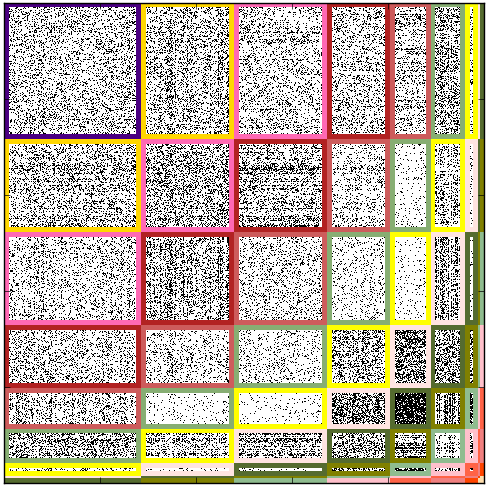
\includegraphics[width=2.94cm, height=3cm]{img/M_g_peaks/figure_6}
	\endminipage
		\minipage{0.17\textwidth}
	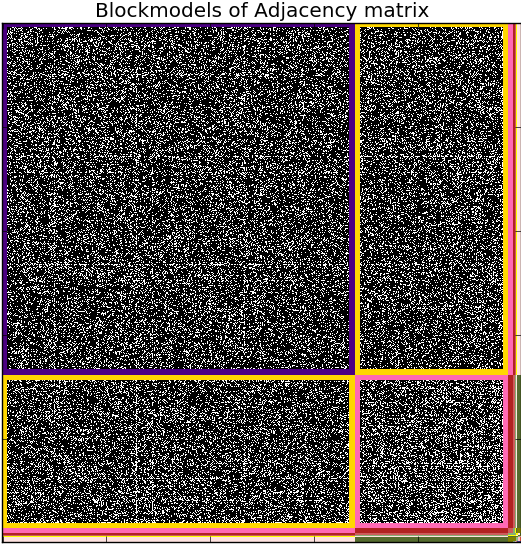
\includegraphics[width=2.94cm, height=3cm]{img/M_g_power_law/figure_6}
	\endminipage
	\minipage{0.17\textwidth}
	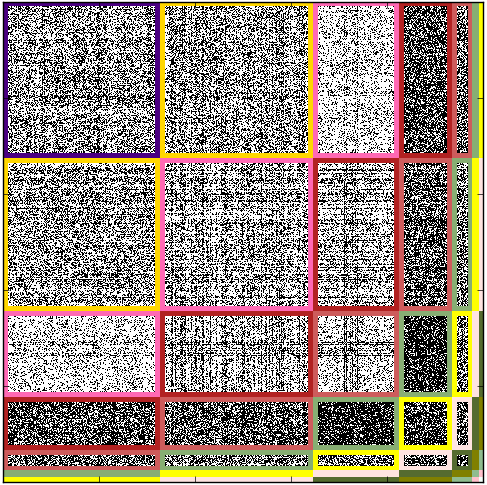
\includegraphics[width=2.94cm, height=3cm]{img/M_g_regular/figure_6}
	\endminipage
	%\vspace{-0.3cm}
    \vspace{0.3cm}
	\minipage{0.16\textwidth}
	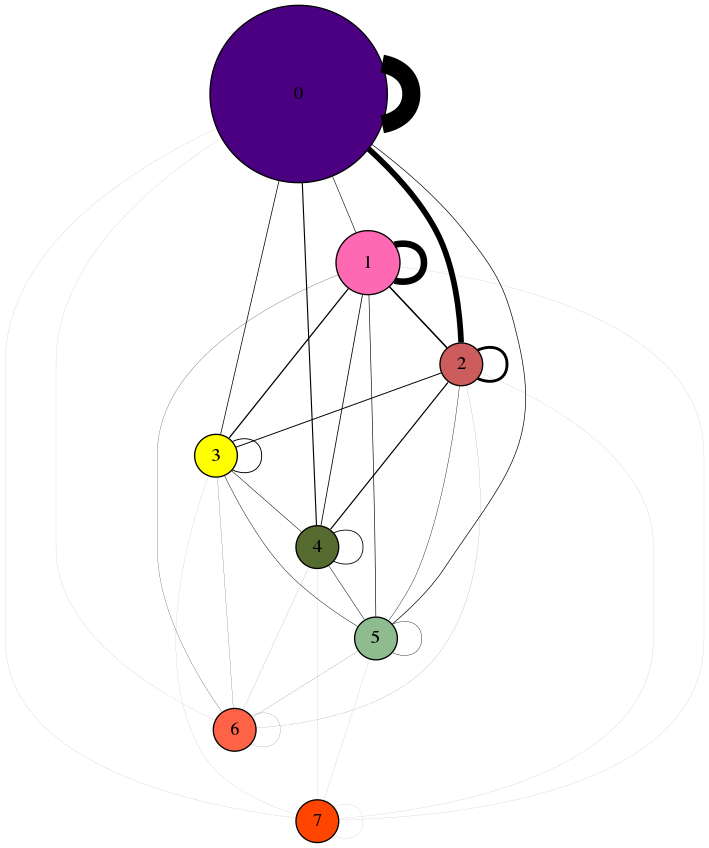
\includegraphics[width=3.5cm, height=4cm]{img/M_g_peaks/graph_dot}
	\endminipage
		\minipage{0.16\textwidth}
	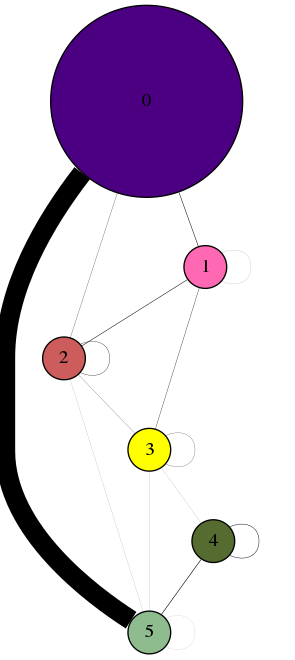
\includegraphics[width=3.5cm, height=4cm]{img/M_g_power_law/graph_dot} 
	\endminipage
	\minipage{0.16\textwidth}
	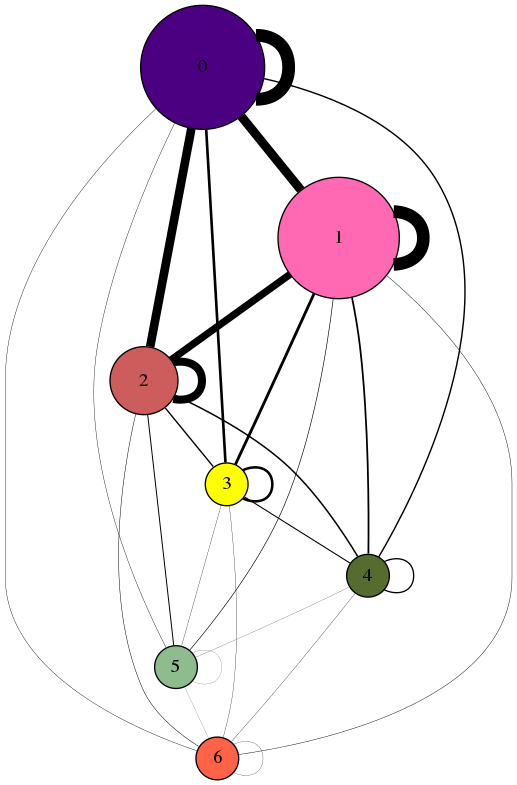
\includegraphics[width=3.5cm, height=4cm]{img/M_g_regular/graph_dot}
	\endminipage
	\caption{Tree examples of generated network in different setting of IMMSB. We we reorder the adjacency matrix (white dot are links, block dot are non-link) in th upper figure, and plot their associated bockmodel structure in the lower part. The block structure is represented in the lower plots where we represent inter-block and intra-block connection by respectively edges ans self-loop.  }
	\label{fig:gen_blocks}
\end{figure}


 We now turn to the burstiness effect.
